%!TEX TS-program = xelatex
%!TEX encoding = UTF-8 Unicode
\documentclass[12pt,a4paper]{article}
\usepackage{geometry} % 設定邊界
\geometry{
  top=1in,
  inner=1in,
  outer=1in,
  bottom=1in,
  headheight=3ex,
  headsep=2ex
}
\usepackage{fontspec} % 允許設定字體
\usepackage{xeCJK} % 分開設置中英文字型
\usepackage{url} % 使用url
\setCJKmainfont{LiHei Pro} % 設定中文字型
\setmainfont{Georgia} % 設定英文字型
\setromanfont{Georgia} % 字型
\setmonofont{Courier New}
\linespread{1.2}\selectfont % 行距
\XeTeXlinebreaklocale "zh" % 針對中文自動換行
\XeTeXlinebreakskip = 0pt plus 1pt % 字與字之間加入0pt至1pt的間距,確保左右對整齊
\parindent 0em % 段落縮進
\setlength{\parskip}{20pt} % 段落之間的距離

\title{\huge 影像處理 Assignment4 - Hough Transform} % 設置標題,使用巨大字體
\author{姓名:吳嘉偉\quad 學號:5105056013\quad 日期:2018/01/13} % 設置作者
\date{} % 設置日期
\usepackage{titling}
\setlength{\droptitle}{-8em} % 將標題移動至頁面的上面
\usepackage{listings}

\begin{document}

\clearpage

\maketitle % 顯示標題

\section{灰階處理}

\subsection{把原始彩色影像轉成灰階影像}

{
\fontsize{14pt}{10pt} % 字型大小14pt,字行間距20pt
\selectfont % 生效
先把彩色的影像轉成灰階影像
\begin{figure}[ht]
\centering
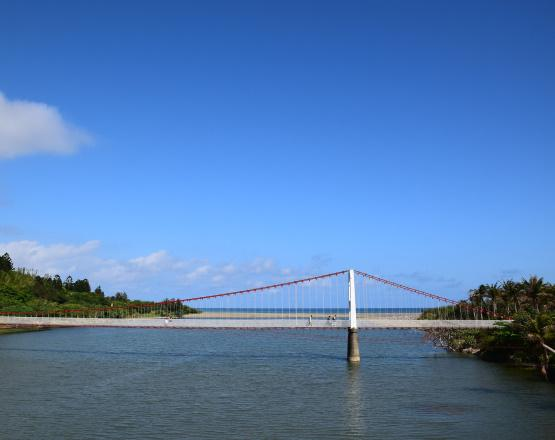
\includegraphics[width=.4\textwidth]{image/bridge.jpg}
\hspace{1cm}
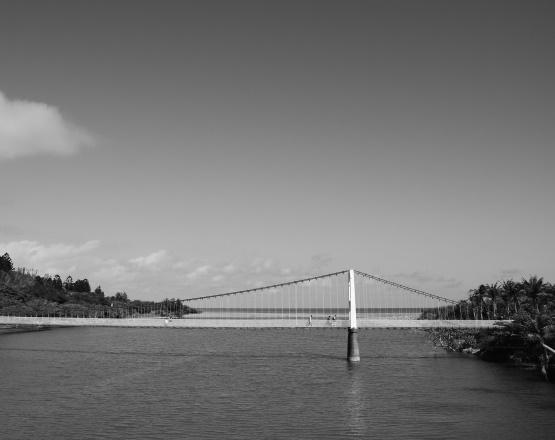
\includegraphics[width=.4\textwidth]{image/gray_image.png}
\caption{Source and Gray Image}%整個標籤
\label{要合併的兩張圖}%整個圖形標籤
\end{figure}
}

\newpage % 新一頁
\subsection{程式碼}

{
\begin{lstlisting}[language=Python]

# 取得並儲存灰階照片
def readGrayImage(name):
    grayImage = cv2.imread(name, cv2.IMREAD_GRAYSCALE)
    savePhoto('gray_image', grayImage)
    return grayImage
    
\end{lstlisting}
}

\section{利用Hough Transform找最長直線}
\subsection{Canny Edge}
{
用Canny Edge找影像的邊緣
\begin{figure}[ht]
\centering
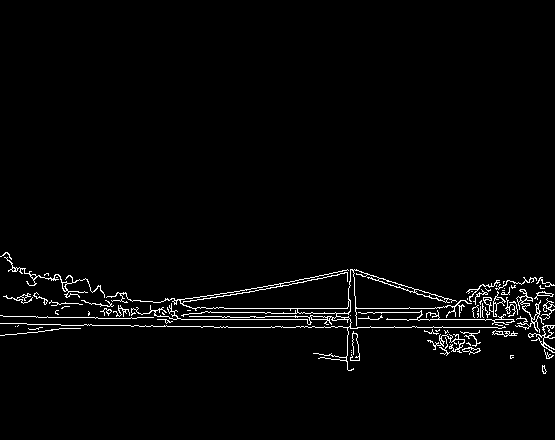
\includegraphics[width=.6\textwidth]{image/canny_image.png}
\caption{Canny Edge Image}%整個標籤
\label{要合併的兩張圖}%整個圖形標籤
\end{figure}

\newpage
程式碼
\begin{lstlisting}[language=Python]
# 使用Canny Edge找出邊緣
def getCannyEdge(image):
    img = cv2.GaussianBlur(image, (3, 3), 0)
    cannyEdgeImage = cv2.Canny(img, 50, 150, apertureSize = 3)
    savePhoto('canny_image', cannyEdgeImage)
    return cannyEdgeImage

\end{lstlisting}
}

\subsection{Hough Transform}
{

\begin{figure}[ht]
\centering
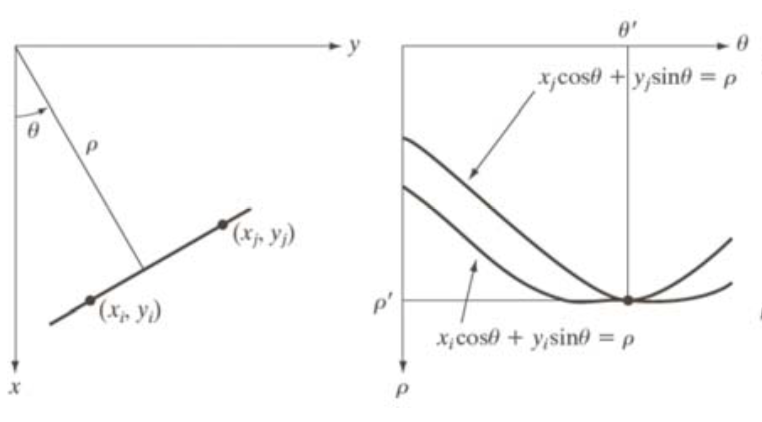
\includegraphics[width=.6\textwidth]{image/houghtransform.jpg}
\caption{Hough Transform Theory}%整個標籤
\label{要合併的兩張圖}%整個圖形標籤
\end{figure}
利用$xcos \theta + ysin \theta = \rho$
\newline
把原本是xy點的座標軸轉換成原點到直線的垂直距離($\rho$)以及與x軸夾角($\theta$)的座標

\begin{figure}[ht]
\centering

\includegraphics[width=.6\textwidth]{image/hough_transform_image.png}
\caption{Hough Transform Image}%整個標籤
\label{要合併的兩張圖}%整個圖形標籤
\end{figure}


程式碼
\begin{lstlisting}[language=Python]
# 取得Hough Transform圖片
def getHoughTransformImage(image, partNumber = 1000):
    height = image.shape[0]
    width = image.shape[1]
    minDistance = 0
    maxDistance = 0
    output_pixels = []

    for y in range(height):
        output_pixels.append([])
        for x in range(width):
            if image[y][x] != 0:
                lineDistance = []
                for count in range(partNumber):
                    angle = math.pi * (2 * count / partNumber - 1)
                    distance = houghTransform(x, y, angle)
                    lineDistance.append(distance)
                    if distance < minDistance:
                        minDistance = distance
                    if distance > maxDistance:
                        maxDistance = distance
                output_pixels[y].append(lineDistance)
            else:
                output_pixels[y].append([])

    height = round(maxDistance - minDistance)
    transData = np.zeros((height, partNumber), np.uint8)
    maxCount = 0

    for i in range(len(output_pixels)):
        row = output_pixels[i]
        for j in range(len(row)):
            line = row[j]
            for k in range(len(line)):
                p = int(line[k] - minDistance)
                transData[p][k] += 1
                if (transData[p][k] > maxCount):
                    maxCount = transData[p][k]

    newImage = np.zeros((height, partNumber, 3), np.uint8)

    for y in range(height):
        for x in range(partNumber):
            newImage[y][x] = int(transData[y][x] * 255 / maxCount)

    savePhoto('hough_transform_image', newImage)
    
\end{lstlisting}
}

\subsection{Longest Line}
{
由於Hough transform把每一個像素(x, y)對應到距離與x軸夾角($\rho$, $\theta$),所以被對應到次數最高的一組($\rho$, $\theta$),就是影像上最長的一條直線
\begin{figure}[ht]
\centering
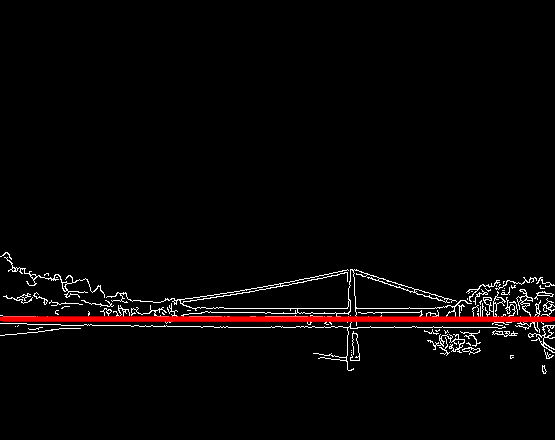
\includegraphics[width=.7\textwidth]{image/finalImage.png}
\caption{Longest Image}%整個標籤
\label{要合併的兩張圖}%整個圖形標籤
\end{figure}

\newpage
程式碼
\begin{lstlisting}[language=Python]
# 畫出最長的直線
def drawLongestLine(cannyImage):
    cdst = cv2.cvtColor(cannyImage, cv2.COLOR_GRAY2BGR)
    lines = cv2.HoughLines(cannyImage, 1, np.pi / 180, 50, None, 50, 10)
    if lines is not None:
        for i in range(0, 1):
            rho = lines[i][0][0]
            theta = lines[i][0][1]
            a = math.cos(theta)
            b = math.sin(theta)
            x0 = a * rho
            y0 = b * rho
            pt1 = (int(x0 + 1000 * (-b)), int(y0 + 1000 * (a)))
            pt2 = (int(x0 - 1000 * (-b)), int(y0 - 1000 * (a)))
            cv2.line(cdst, pt1, pt2, (0, 0, 255), 3, cv2.LINE_AA)
    savePhoto('finalImage', cdst)
    
\end{lstlisting}
}

\end{document}